\section{Background and Related Work}
\label{sec:background}
We now discuss the background and prior work on batching, scheduling, and prefix-aware optimizations.

\subsection{Background}

\subsubsection*{LLM Inference and Attention}
LLM inference proceeds auto-regressively in two phases: prefill and decode. Their latencies are known as \textit{time to first token} (TTFT) and \textit{time between tokens} (TBT), respectively. Each decode step comprises self-attention, Query-Key-Value-Output (QKVO) projections, and Multi-Layer Perceptron (MLP) layers. Self-attention captures global token dependencies as:
\[
\text{Attention}(\mathbf{Q}, \mathbf{K}, \mathbf{V}) = \text{softmax}\left(\frac{\mathbf{Q}\mathbf{K}^T}{\sqrt{d}}\right)\mathbf{V}
\]
where $d$ denotes the head dimension. During the decode phase, the query $\mathbf{Q}$ of the current token attends to all prior keys $\mathbf{K}$ and values $\mathbf{V}$. These are cached in GPU memory as the \textbf{KV cache}, eliminating redundant computation at the cost of increased memory usage. The asymmetry between prefill and decode, together with the growing memory footprint of the KV cache, motivates much of the prior work.

\vspace{-10pt}

\subsubsection*{GPU Execution Model}
GPUs are hierarchically organized for parallelism across hundreds of thousands of threads. The basic compute unit is the Streaming Multiprocessor (SM), and modern GPUs typically contain a few hundred SMs. Each SM includes an L1 cache, shared memory, tensor cores for matrix multiplication (GEMM), and execution units. SMs access global memory through a shared L2 cache. This hierarchy, from small, fast on-chip memory to large, high-latency global memory, is critical for LLM serving, as KV cache access patterns directly influence memory bandwidth utilization. Like CPUs, GPUs use hardware prefetching and benefit from regular, sequential memory access patterns~\cite{Peng_2017}.

\vspace{-7pt}

\subsection{Related Work}
\subsubsection*{Batching and Scheduling}
vLLM~\cite{kwon2023efficient} adopts a first-come, first-served (FCFS) scheduling policy as a practical baseline for LLM serving. Sarathi-Serve~\cite{agrawal2024tamingthroughputlatencytradeoffllm} reduces prefill-decode interference through \textit{chunked prefills} and stall-free batching, while DistServe~\cite{zhong2024distservedisaggregatingprefilldecoding} eliminates it by disaggregating the two phases across GPUs. At the kernel level, POD-Attention~\cite{Kamath_2025} overlaps prefill and decode on a single GPU via fused attention with SM-aware scheduling, and Bullet~\cite{lin2025boostingllmservingspatialtemporal} enables fine-grained resource sharing through dynamic SM allocation. At the request level, BucketServe~\cite{zheng2025bucketservebucketbaseddynamicbatching} groups requests by sequence length to improve batching efficiency, and \citet{pang2025optimizing} dynamically adapts the batch size to runtime constraints. Complementary to prior work, \textit{\Feather operates at the scheduler level and learns when to stop batch construction based on prefix homogeneity, introducing a scheduling signal not explicitly exploited in existing systems.}

\vspace{-7pt}

\subsubsection*{Prefix Sharing}
Many real-world LLM workloads~\cite{brown2020languagemodelsfewshotlearners,NEURIPS2021_5c049256,thebigpromptlibrary,lewis2021retrievalaugmentedgenerationknowledgeintensivenlp} exhibit substantial prefix overlap, and enabling KV cache reuse avoids redundant computation and reduces memory footprint. However, realizing these benefits requires coordination between serving and memory management. SGLang \cite{zheng2024sglangefficientexecutionstructured} formalizes prefix sharing via \textit{RadixAttention}, which uses a radix tree to hierarchically organize token sequences, and enables KV reuse across shared prefixes. Similarly, vLLM~\cite{kwon2023efficient} implements prefix caching~\cite{vllm_prefix_caching_docs} using a Merkle-tree-inspired hashing scheme (Figure~\ref{fig:vllm_merkle_tree_example}), where each KV block hash depends on its tokens and preceding prefix hashes, enabling reuse when hash sequences match. BatchLLM~\cite{zheng2025batchllmoptimizinglargebatched} targets large offline workloads by grouping prefix-sharing requests and reordering them to maximize KV reuse. BlendServe~\cite{zhao2024blendserveoptimizingofflineinference} combines a resource-aware prefix tree with scheduling to jointly optimize prefix reuse and compute–memory demand. \Feather adopts a lightweight design: \textit{it uses chunked hashing over radix trees or full hash chains, reducing CPU overhead and steering batch construction toward prefix-homogeneous groups in online and offline settings.}

\vspace{-7pt}

\begin{figure}[t]
    \centering
    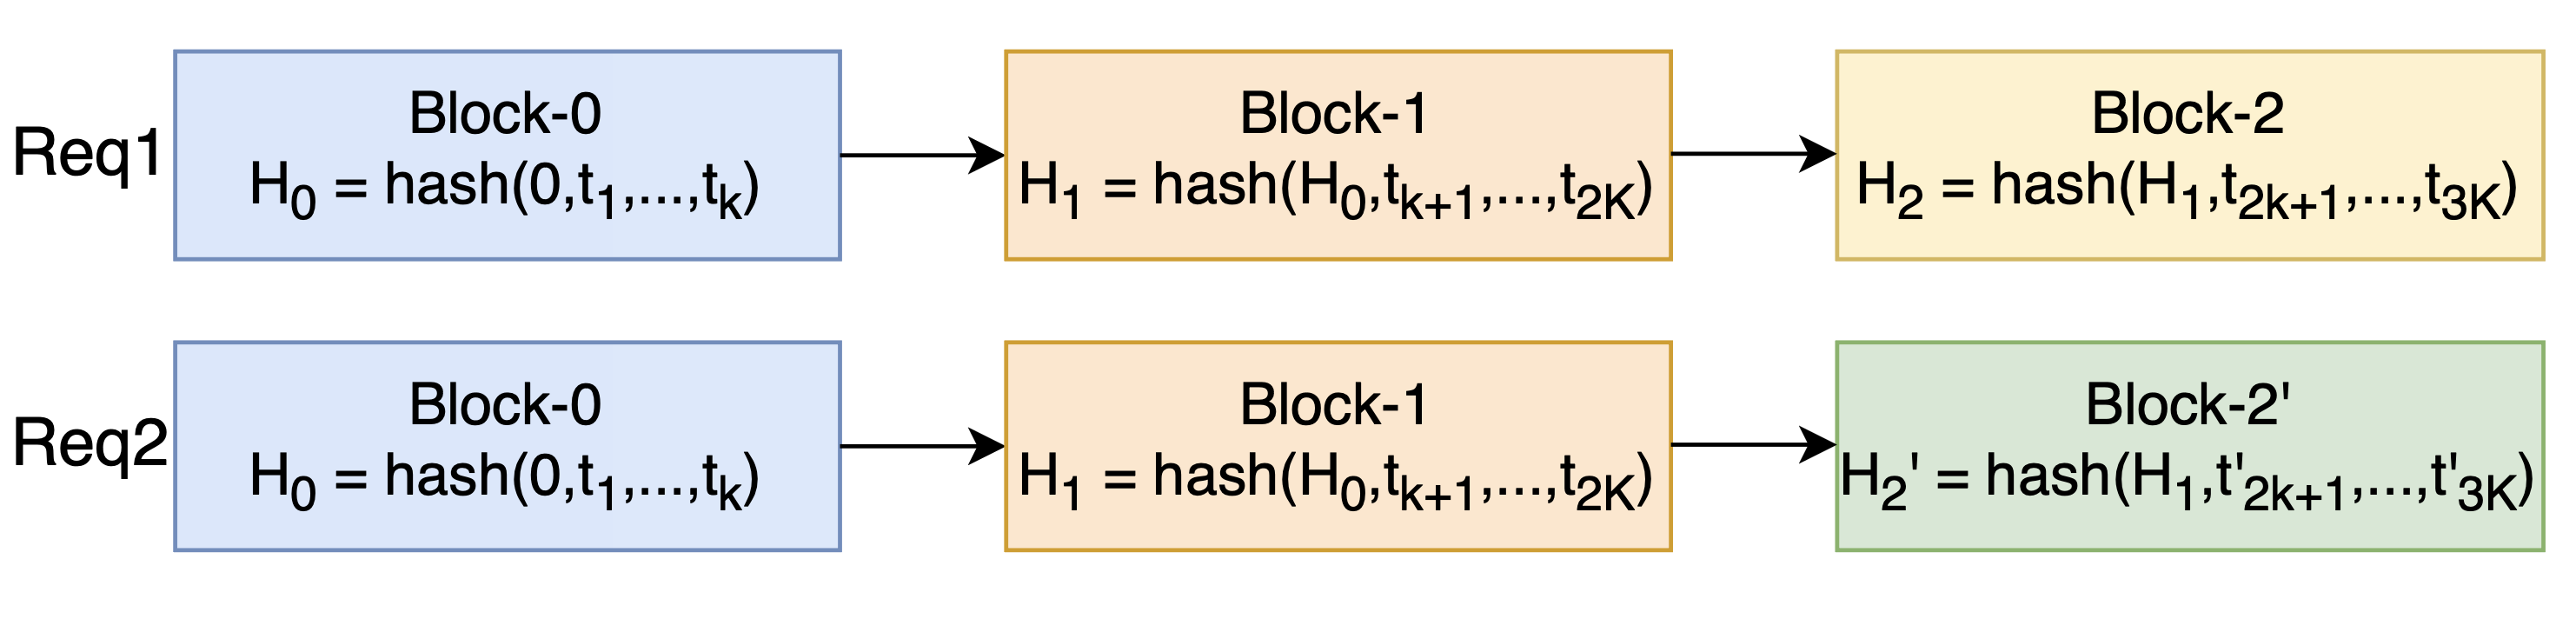
\includegraphics[width=\linewidth]{illustration_images/vllm_merkle_tree.png}
    \caption{An Example of a vLLM Merkle Tree}
    \label{fig:vllm_merkle_tree_example}
    \vspace{-18pt}
\end{figure}

\subsubsection*{Prefix-Aware Attention Kernels}
Prior work~\cite{yi2026pat,yao2025deftdecodingflashtreeattention,ye2024chunkattentionefficientselfattentionprefixaware,MLSYS2025_96894468} also optimizes attention kernels by grouping queries with shared prefixes to load KV blocks once and reuse them across queries. These approaches, however, rely on GPU-specific kernel designs. In contrast, \textit{\Feather improves inputs to the existing attention kernels by constructing prefix-homogeneous batches upfront, making it hardware-agnostic and naturally composable with kernel-level techniques.}